This section provides the reader with an overview of the RV8 robot work cell. The primary operational aspects of the product, from the perspective of end users, maintainers and administrators, are defined here. The key features and functions found in the work cell, as well as critical user interactions are described in detail below.

\subsection{Features \& Functions}
The RV8 work cell will specialize in precisely marking on an object incorporating all aspects of the robot arm and linear rail. It will perform these operations through the use of a compressor which will be connected to the PLC. The vertical robot initially has 6 axis, with a linear rail acting as the 7th axis. The robot will precisely paint, where the system will send signal to the compressor which will output the paint on a plastic sheet. While performing the operation, several safety features will be implemented, such as emergency stops, and industrial light towers. The integrated components of the work cell are the Programmable Logic Controller (PLC), host PC, and a CR800 handheld controller.

\subsection{External Inputs \& Outputs}
\begin{table}[H]
\resizebox{\textwidth}{!}{
\begin{tabular}{|l|l|l|l|}
\hline
 \textbf{Name} & \textbf{Description} & \textbf{Use}\\ \hline
 Air brush \& compressor & System output & Sprays the paint from the air brush \\ \hline
 Presence Detection & System input & Detects motion within the work cell  \\ \hline
 Emergency Stops & User input & Stops the operation of the robot arm \\ \hline
 Industrial Light Tower & System output & Indicates the state of the work cell  \\ \hline
Inductive Switches & System input & Indicates the end limits of linear rail \\ \hline
\end{tabular}}
\caption{Overview of external inputs and outputs}
\end{table}

\subsection{Product Interfaces}
Specify what all operational (visible) interfaces look like to your end-user, administrator, maintainer, etc. Show sample/mocked-up screen shots, graphics of buttons, panels, etc. Refer to the critical external inputs and outputs described in the paragraph above.

\begin{figure}[h!]
	\centering
   	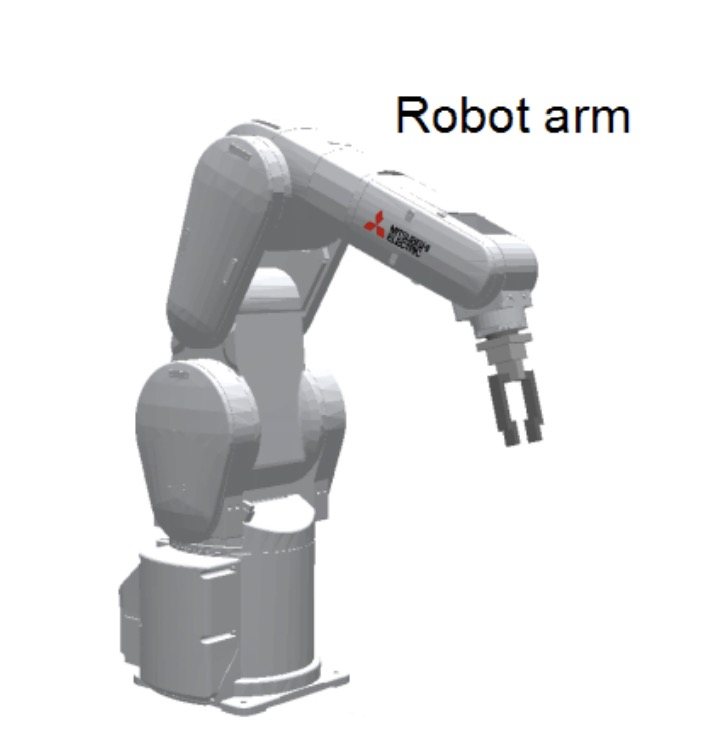
\includegraphics[width=0.30\textwidth]{images/RobotArm.jpg}
    \caption{Robot arm of RV8-CRL
    }
\end{figure}
\begin{figure}[h!]
	\centering
   	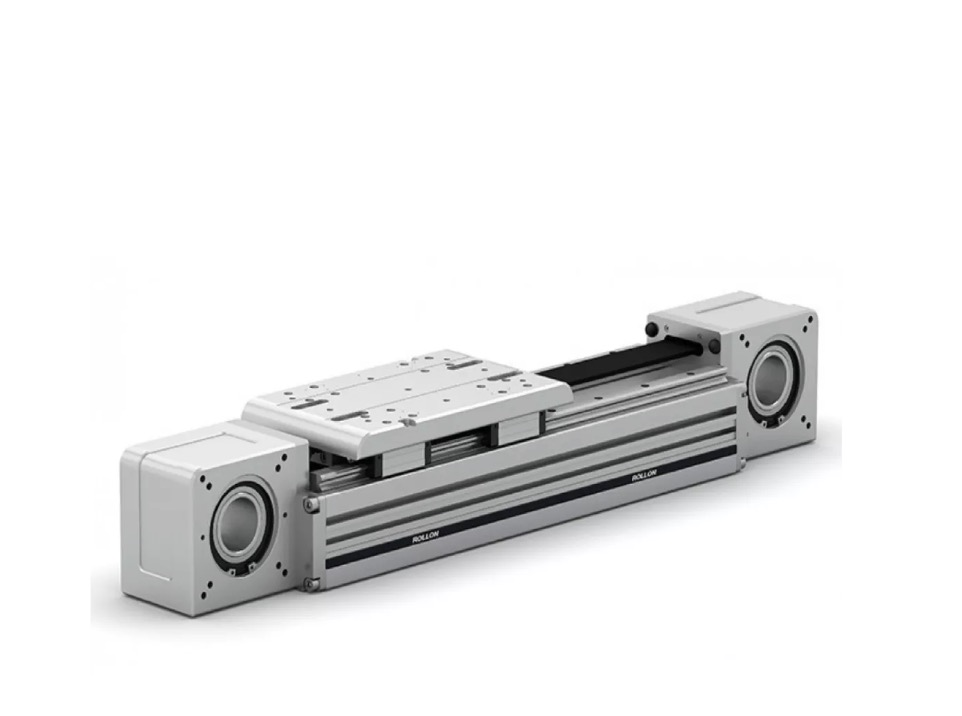
\includegraphics[width=0.40\textwidth]{images/LinearRail.jpg}
    \caption{Linear rail}
\end{figure}

\begin{figure}[h!]
	\centering
   	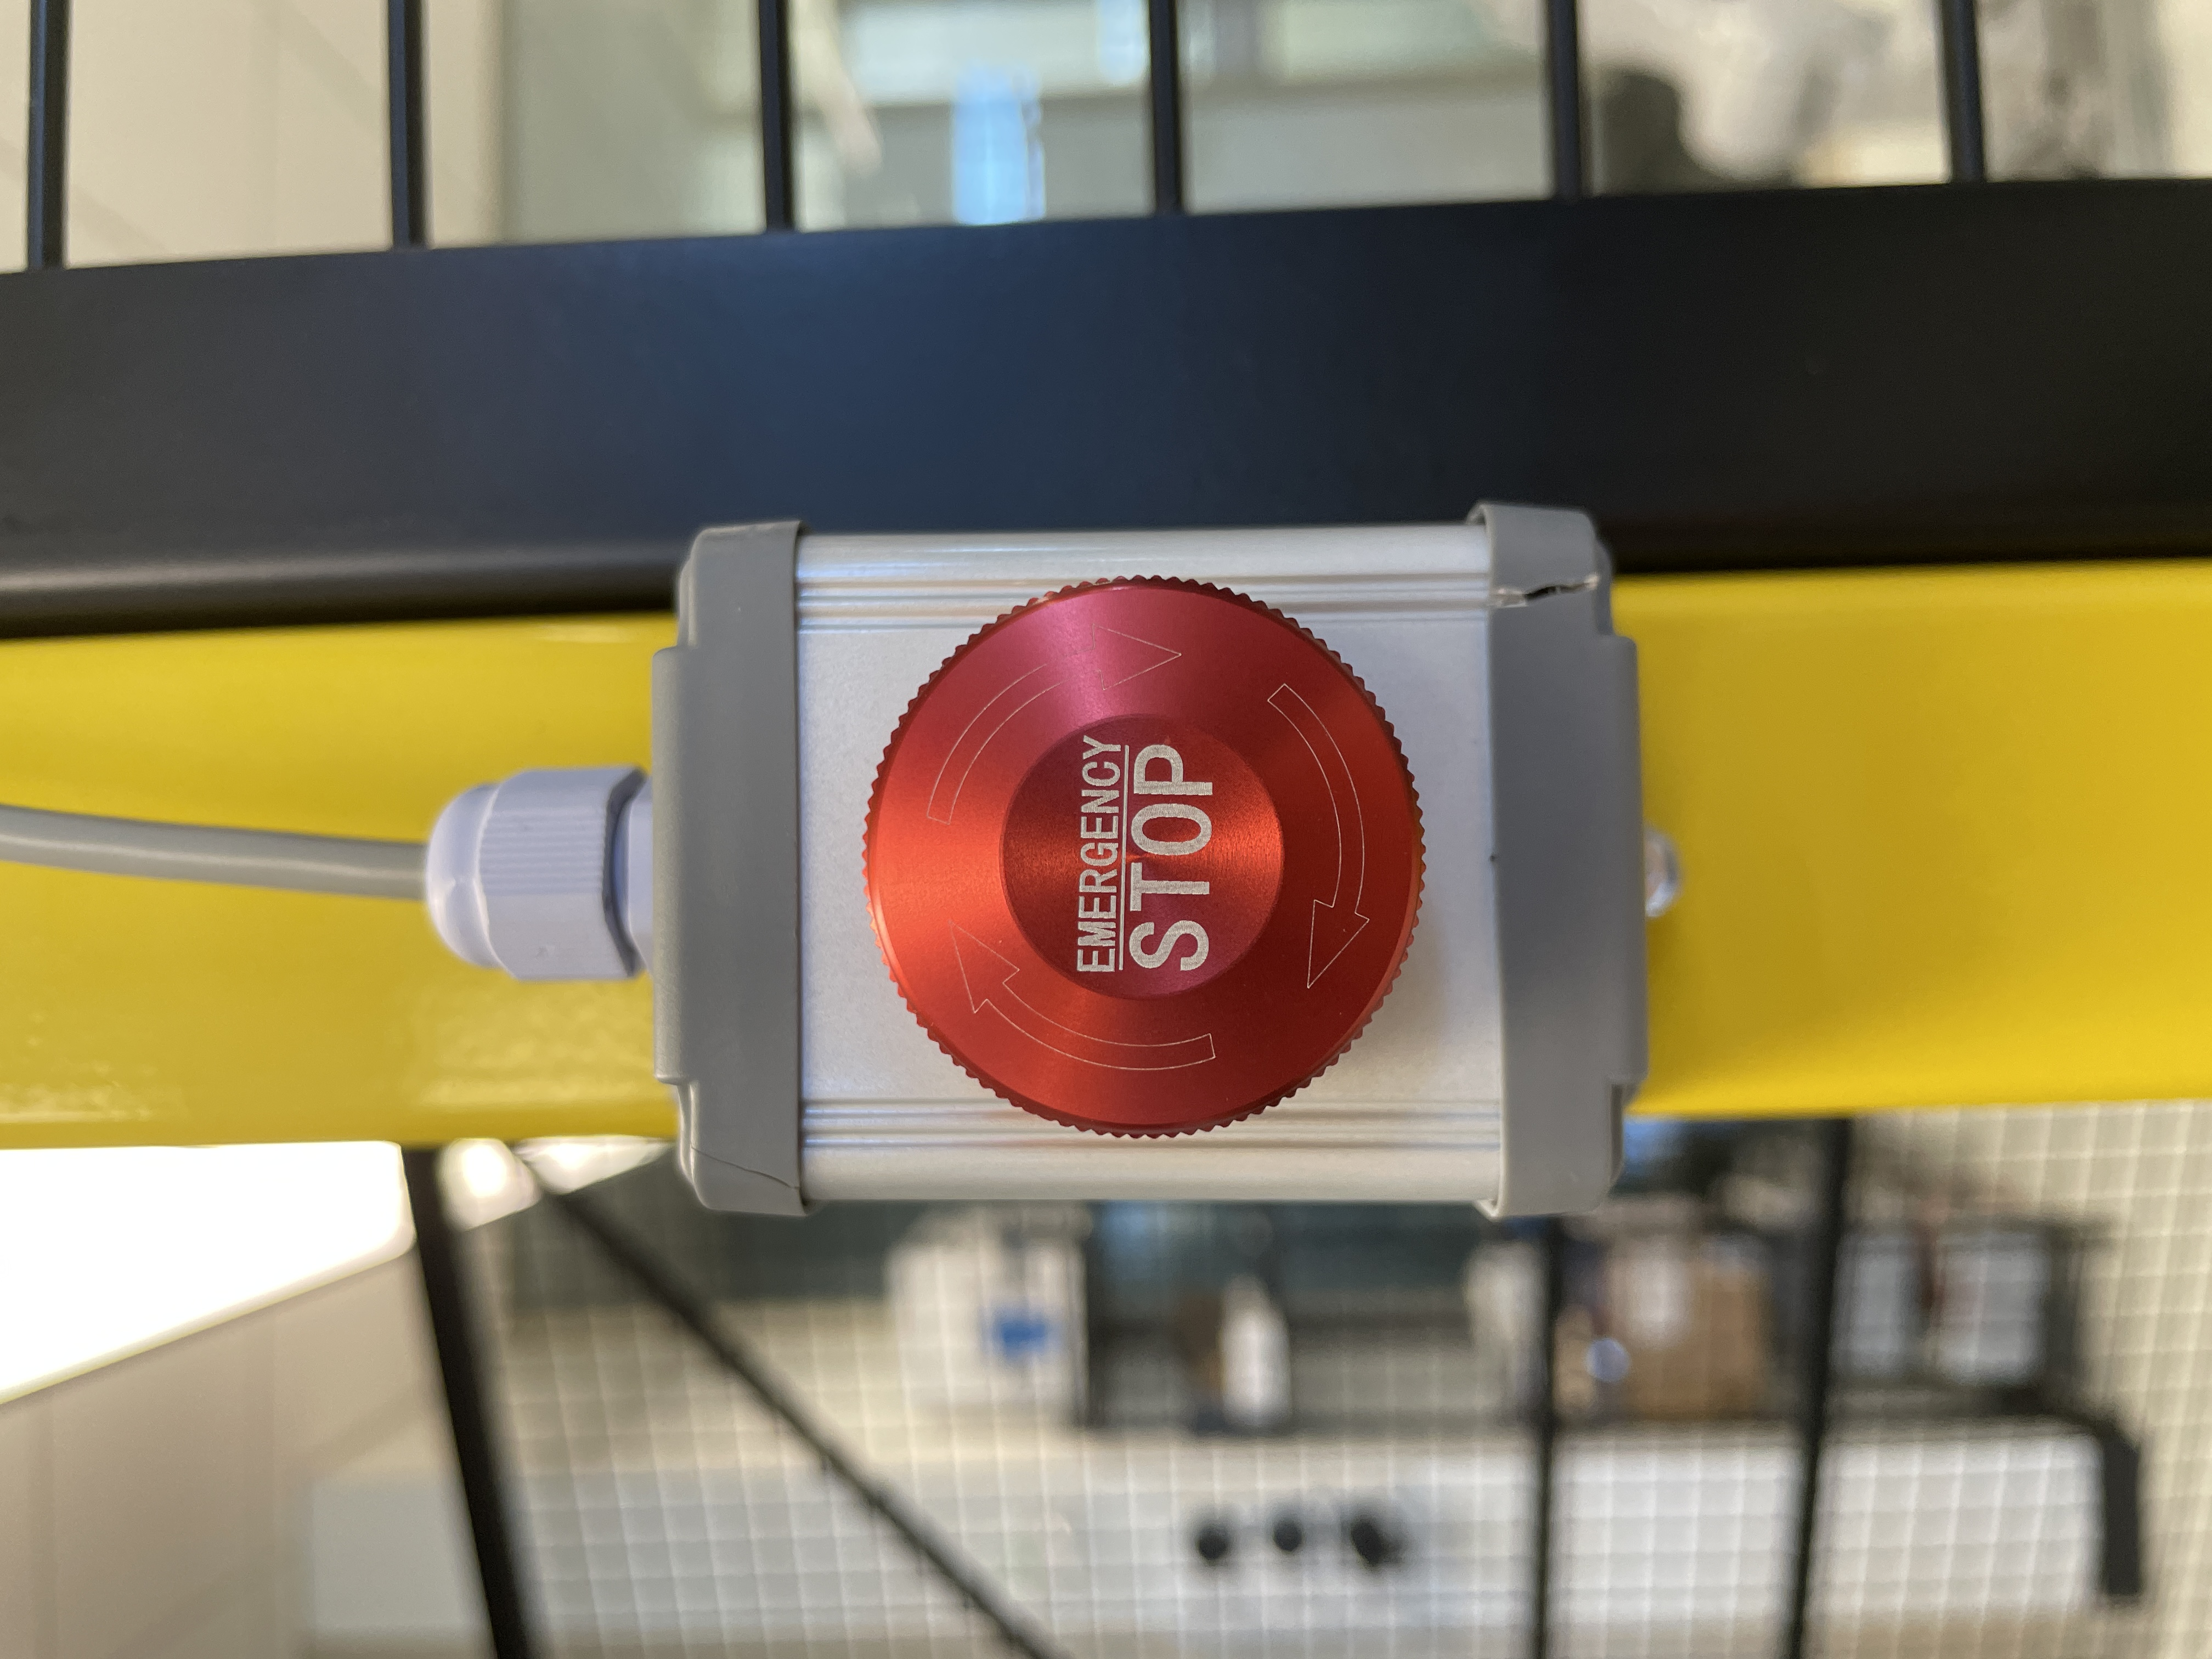
\includegraphics[width=0.40\textwidth, angle = -90]{images/EStop.JPG}
    \caption{Emergency stop}
\end{figure}

\begin{figure}[h!]
	\centering
   	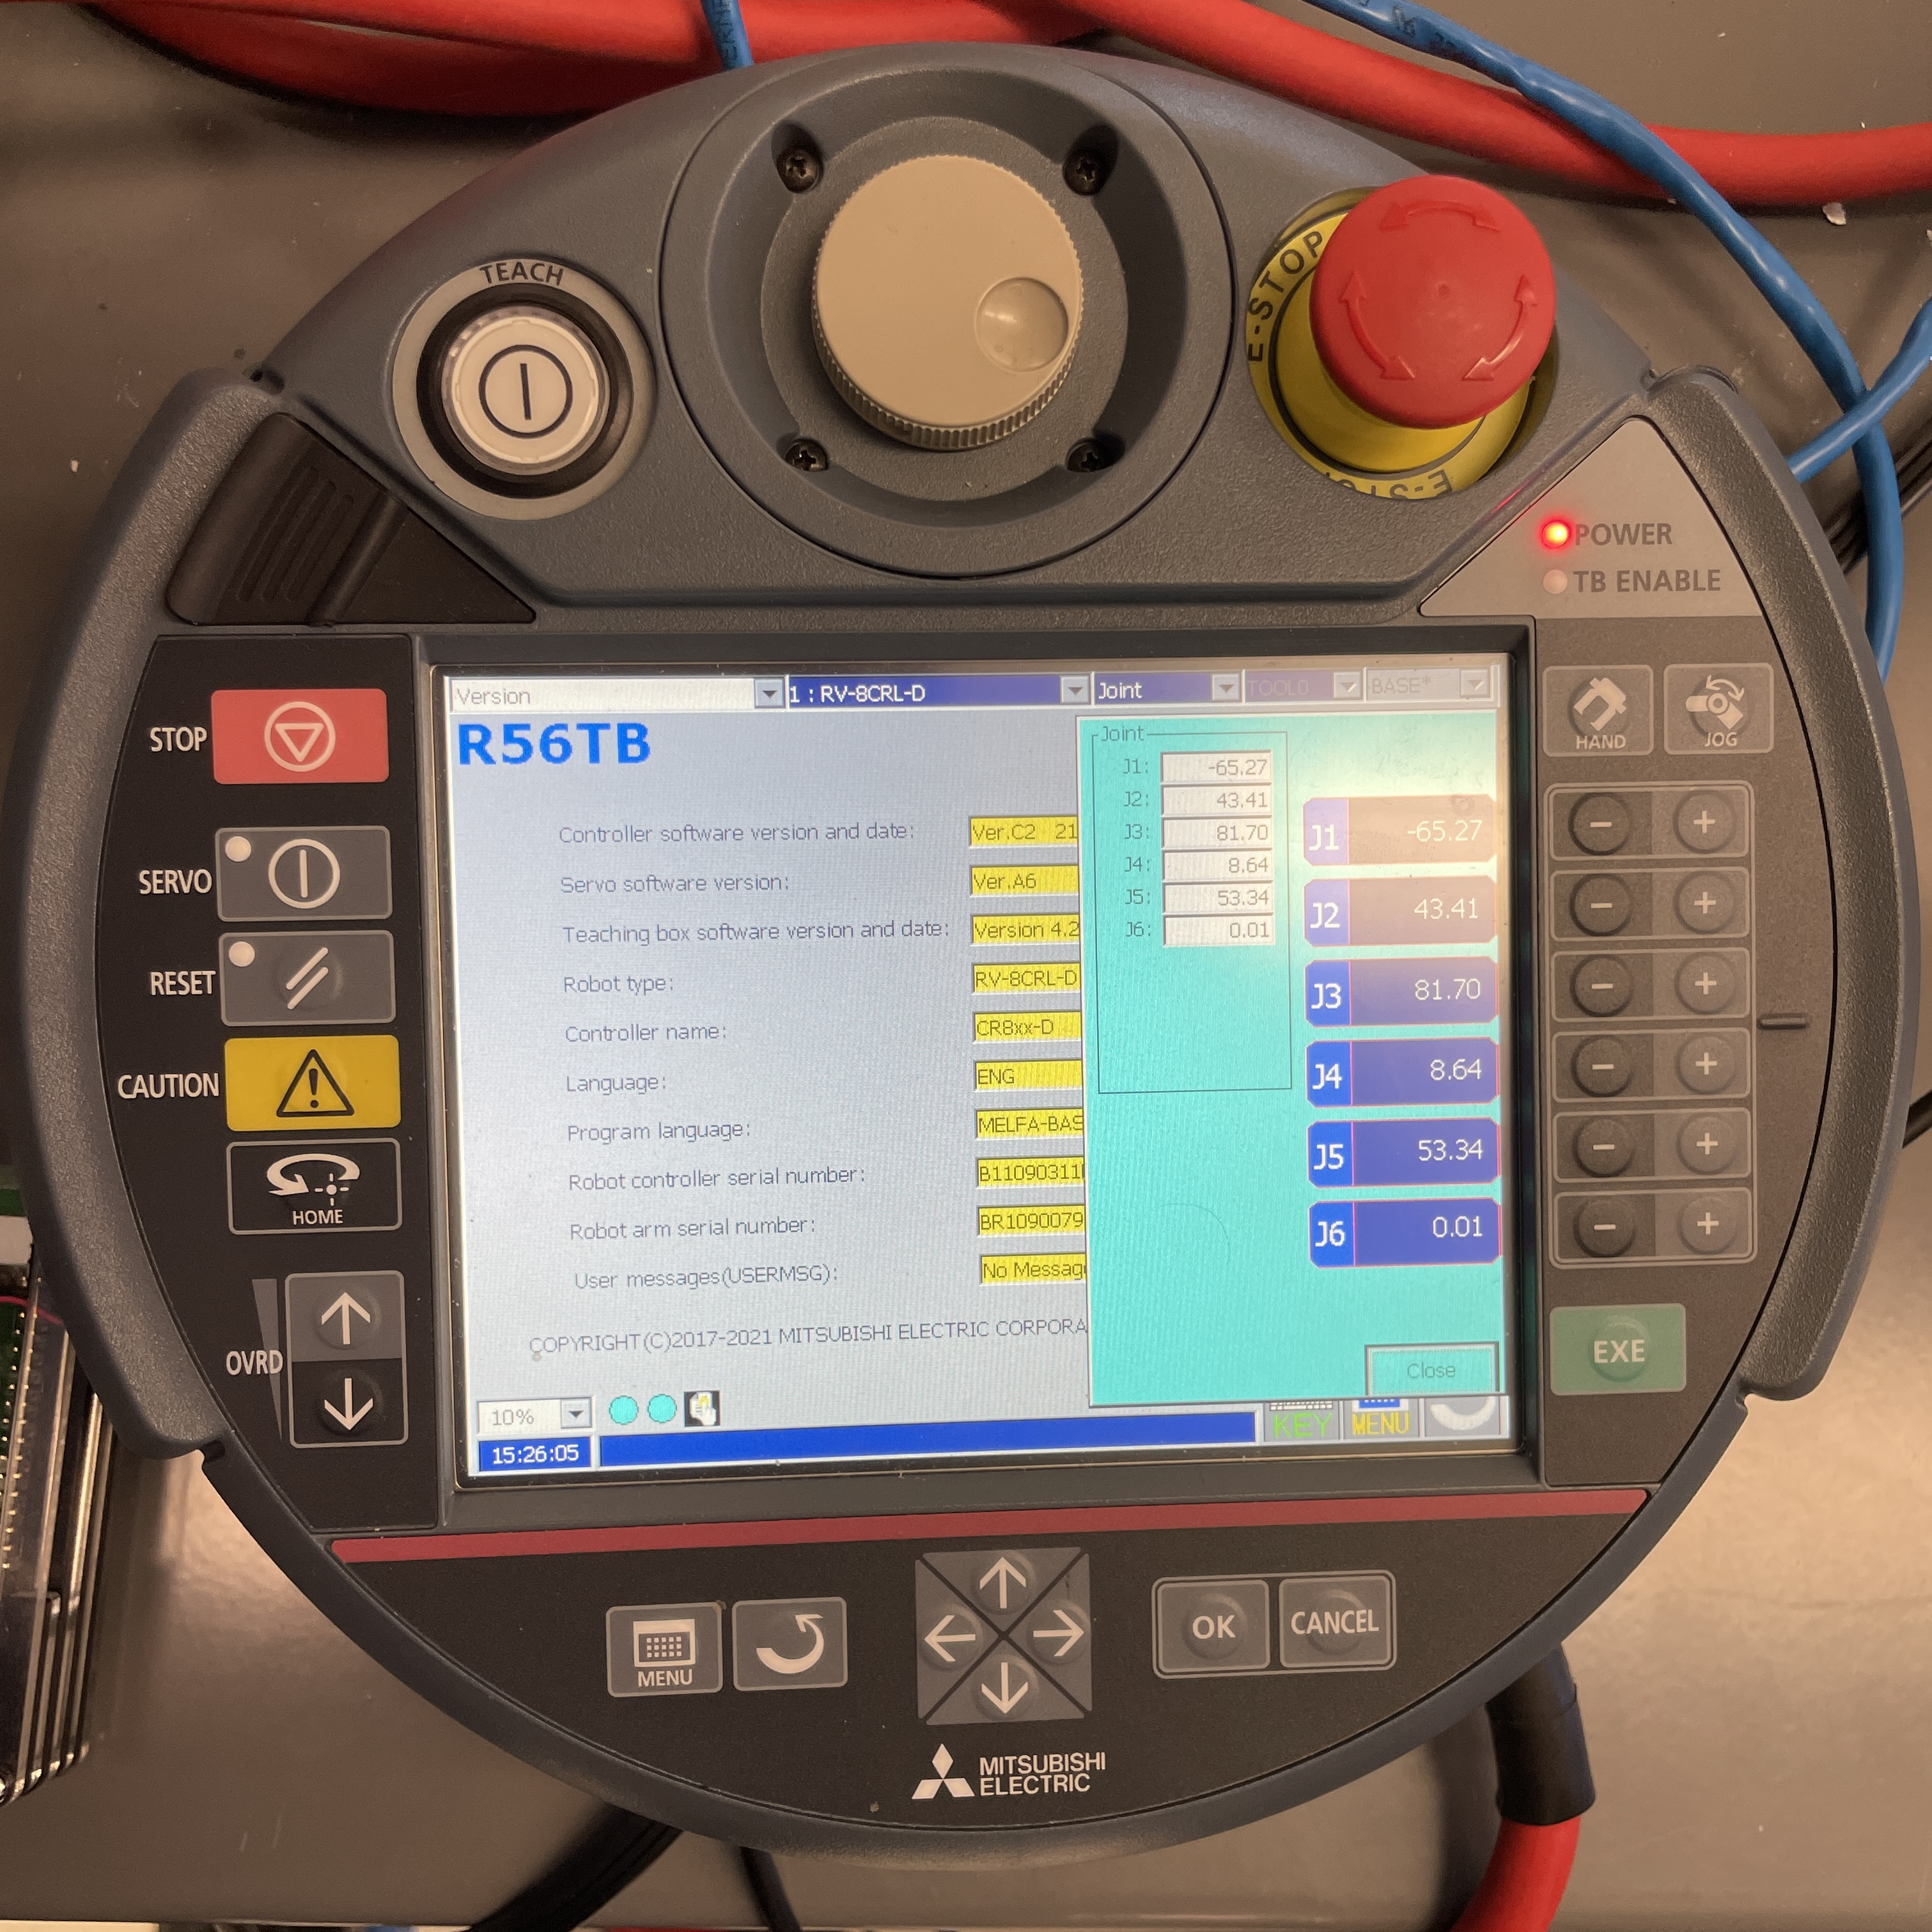
\includegraphics[width=0.40\textwidth]{images/CR800.jpg}
    \caption{CR800 controller}
\end{figure}



